\chapter{Observing with SALSA}
It is important to be well prepared before you start observing with SALSA.
Time is not only limited, because of the Earth's rotation some objects on the
sky can only be seen during a specific part of the day.  Please try to get a
clear understanding of what you want to do before using the telescope.  In this
chapter we describe what can be observed, how to control the telescope, and how
to extract your measurements. We strongly recommend you to read this document
before starting your first observations. 

\emph{Please note:} after your observations, please put the telescope in the
\verb!Stow! position. This is done by selecting \verb!Stow! from the drop-down 
list of targets in the control program and clicking \verb!Track!. In the stow
position the telescopes are less vurlnerable to high wind speeds which may
cause mechanical damage.

\section{What can be observed with SALSA?}
Although the SALSA system was primarily designed for observing galactic
hydrogen there are a few other ways to use the telescope. In the following
subsections we describe the ideas we have tested so far. More projects
will be added as we find the time.

\subsection{The Milky Way}
Most users of SALSA aim to detect emission from hydrogen gas in our galaxy the
Milky Way.  The aim here is to detect emission from hydrogen gas emitting at
frequencies close to 1420.4\,MHz.  This is what the SALSA website and control
program was designed for and most of the available documentation is related to
this particular project. For an extended description of this project, see the
document \emph{Mapping the Milky Way} available via the SALSA website.

\subsection{The Sun}
The Sun is a bright radio source and can be detected easily with SALSA. 
Observations of the Sun can be used to determine the reception pattern
of the SALSA antenna. More information about this project can be found
in the document \emph{Measure the beam of SALSA}, available via the SALSA
website.

\subsection{GNSS satellites}

Progress in space sciences and exploration of the universe, begun in 1960's, caused that
many satellites started to appear at the Earth's orbit at altitudes from 2000 to 20 000~km. 
Such artificial objects are used in many different fields of science and engineering such as 
telecommunication, meteorology, environmental monitoring or navigation. The latter is realized through 
a so-called Global Navigation Satellite Systems (GNSS). SALSA users are able to detect signals emitted from 
GNSS satellites. More information about this project can be found in the document 
\emph{GNSS signal spectra with SALSA}, available at the SALSA website.

%\subsection{Cassiopeia A}
%Cassiopeia A is a bright radio source and should be observable
%with SALSA in a way similar to how we observe the Sun. We have not yet
%had the time to verify that we can indeed detect Cas. A, but as soon
%as we do we will provide instructions on the SALSA website. 
%
%\subsection{The Andromeda galaxy}
%The Andromeda galaxy contains a lot of neutral hydrogen, just like the Milky
%Way. In theory we should be able to detect hydrogen emission from Andromeda and
%derive the rotational speed of the galactic disc. However, because the galaxy
%is much further away than the gas clouds in the Milky Way, we will probably
%need to measure for many hours. Unfortunately, SALSA is, for technical reasons,
%not yet capable of doing such long measurements. We aim to improve the system
%in the future to make it possible to detect Andromeda, and when we have
%confirmed that it works we will provide a set of instructions on the SALSA
%website.

\section{When can SALSA see my desired target?}
Not all celestial objects are visible from Onsala, and some are only above the
horizon for a short time each day. Before your observations it is good to
prepare to make sure that your target is indeed visible. More information about
how to do this can be found in Appendix \ref{app:coord}. Note that this
appendix also includes a list of galactic coordinates which are always visible
from Onsala, these may be a good start if mapping the Milky Way. 

Another way to find out what you can see with SALSA at a specific time is to
install the free software \emph{Stellarium}, available at
http://stellarium.org/.  Tell the program that you are in Onsala (or in
Kungsbacka, which the program knows about and is close enough to Onsala), and
select a date and time.  The program will then predict how the sky will look.
Note that you can display coordinate grids within Stellarium, and both Galactic
and Equatorial coordinates are supported.

\section{Connecting to SALSA} 
\label{sect:connect}
The SALSA telescopes are controlled from a computer in Onsala. If you are at
the observatory, then you can login to the computer directly. However, most
observations are done remotely via internet. To control SALSA you thus need to
login remotely to a computer in Onsala. This remote control has been tested
on Windows, Mac OS X and Linux so you should be able to connect using any 
computer. There are two common ways to connect to the computer in Onsala:

\begin{itemize}
	\item{\emph{In your browser.} This is the most common way to control a
			SALSA telescope. No software is needed except for a recent 
			webbrowser. You find the links to the browser login pages for
			the telescopes at the page \emph{Observe} at the SALSA webpage.
			
		Note: Your browser will complain that the connection is \emph{untrusted},
			because we have no certificate for the SALSA computers. Please
			ignore this warning to login to the telescope. To do so in Firefox,
			select \emph{I Understand The Risk, Add Exception, Confirm
			Exception}. In Safari: click \emph{continue}. In Explorer: click
			\emph{continue}.  Once connected you may start the control program by
			clicking on the SALSA-shortcut on the virtual desktop, or starting
		a terminal and typing SALSA. }

\item{\emph{In the terminal.} If you are used to working in the terminal you
		may login through SSH with graphics support using the command \emph{ssh
		-X username@computer}, where computer is either vale.oso.chalmers.se or
		brage.oso.chalmers.se depending on what you booked.  You may then start
		the control program from the terminal with the command {\tt  SALSA}.}
\end{itemize}

\subsection{Ending your session}
When you are done observing, please close the control program using the
\emph{x} in the upper right corner. Then close your connection to the SALSA
computer. If you are connected using the browser, you close your connection by
closing the virtual desktop, e.g. by clicking the button in the upper corner. 
If you are connected via SSH in a terminal, you close your connection by 
typing {\tt exit}.

\emph{Please note:} after your observations, please put the telescope in the
\verb!Stow! position. This is done by selecting \verb!Stow! from the drop-down 
list of targets in the control program and clicking \verb!Track!. In the stow
position the telescopes are less vurlnerable to high wind speeds which may
cause mechanical damage.

\subsection{Troubleshooting}
Do you have trouble connecting to the telescope? Before contacting support,
please check the three most common issues:
\begin{itemize} 
\item The password for the control computer may be different from the password
you chose for the webpage (to make bookings). To log in to a control computer
you need to use your \emph{telescope password} which you can find under
\emph{my account} on the SALSA website.
\item Make sure you connect to the right computer. The host adress is different
for different telecopes, but it has always the same format. For example, if
you have booked the telescope \emph{vale} then the computer is
\emph{vale.oso.chalmers.se}. If you have booked the telescope \emph{brage}
then the computer is \emph{brage.oso.chalmers.se}. 
\item Make sure you have made a reservation at the correct time. The booking
	system shows all times in your selected timezone. You may check the time
	right now in your selected timezone by looking at the clock on the SALSA
	website. 
\end{itemize}

\section{The telescope control program} 
\label{sect-control}
When you are logged in on a telescope computer you can start the control
program, by either clicking the icon \emph{SALSA} on your desktop, or by
running \emph{SALSA} in a terminal.  You should \footnote{Sometimes the window
	takes more than 10 seconds to appear, be patient. If you do not see any
window, try again and wait up to 30 seconds. If you still see nothing, please
contact support as described on the SALSA website.} now see the main control
program looking very similar to Fig. \ref{fig:controlstart}. 
\begin{figure}[ht]
\begin{center}
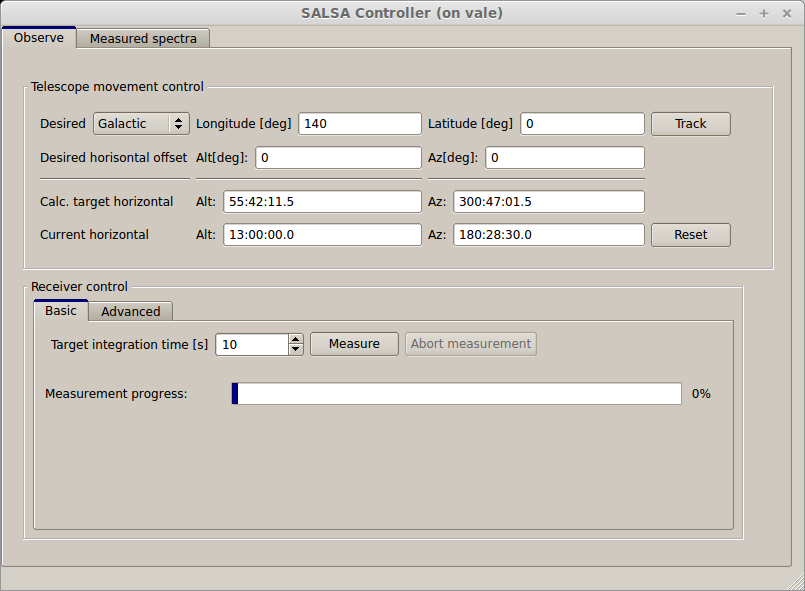
\includegraphics[width=\textwidth]{../figures/Controller_start.png}
\end{center}
\caption{Startup display of the SALSA control program.}
\label{fig:controlstart}
\end{figure}
The control program is used to move the telescope and to record measurements.
We will start by describing how to move the telescope, and then we describe
how to record data.

\subsection{Movement control: To point the telescope}
The startup display of the SALSA control program contains a box labelled
\emph{Telescope movement control}. This box contains four rows of white
fields. We now describe the purpose of these fields in detail. 

The first two rows are for user input, i.e. you may enter values here.  The
first row is labelled \emph{Desired}. This row must be specified by you, this
is where you specify where you want the telescope to point. Different
coordinate systems are valid, but Galactic coordinates are most common since
they are used when observing galactic hydrogen. A few special objects can also
be selected directly, for example the Sun.

The second row is labelled
\emph{Desired horizontal offset}. This row is only used in special cases, for
example when doing beam measurments, and should be left at 0 for most
observations, e.g. for galactic hydrogen. 

The rows three and four are for display only, i.e. you do not enter any values
here.  The third row is labelled \emph{Calc. target horizontal}. This row
displays the target local (altitude-azimuth) coordinates as calculated by the
control program given the desired coordinates you have entered (including a
possible offset from the second row). Note that the coordinates are changing
as the current pointing is re-calculated every second. These calculations
are done automatically by the program. 

The fourth and last coordinate row shows the current local coordinates, i.e.
where the antenna is pointing at this very moment. Once you tell the antenna
to move, see below, it will start moving until the current coordinates (row four)
is the same as (or very close to) the position calculated in row three.

\subsubsection{Tracking}
Tracking means to track or \emph{follow} a specific object or coordinate on the
sky. This means that the telescope needs to move to correct for the movement of
the Earth (the rotation is about 0.25$^\circ$ per minute). Once you have
specified the target coordinates correctly, click on the button {\tt Track}.
The telescope will now start moving, see Fig. \ref{fig:controlmove}, and will
keep calculating and moving to follow your target on the sky until you tell it
to stop by pressing the button {\tt Stop}.  Don't forget to look at the webcam
at the SALSA website to check that the telescope is indeed moving.  Once you
reach the target you will probably not notice the minor tracking movement by
eye, but if you look carefully you will see the \emph{Current} coordinates will
changing slightly over time to follow the change in the calculated position.
Note that it may take up to a few minutes to reach your desired position if you
started pointing far away on the sky. Measuring while moving will produce
nonsense data.  
\begin{figure}[ht]
\begin{center}
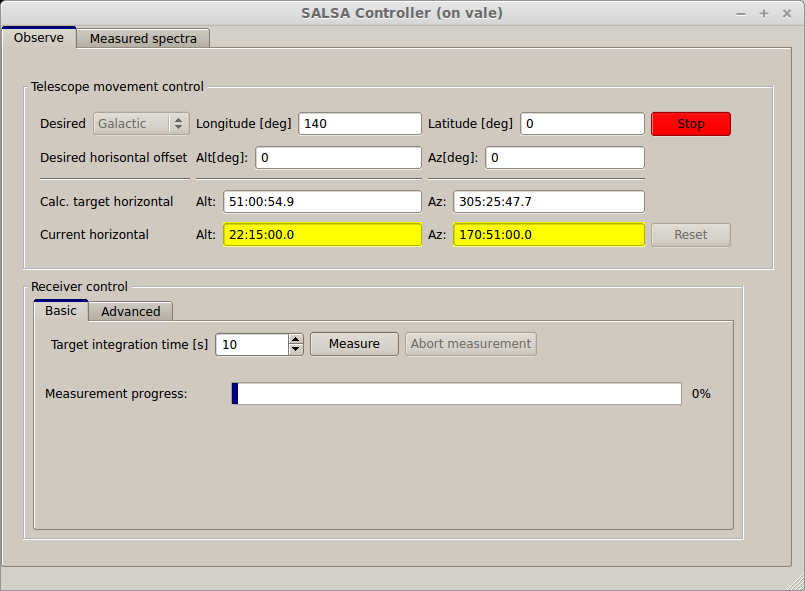
\includegraphics[width=\textwidth]{../figures/Controller_move.png}
\end{center}
\caption{The telescope control program display when the telescope is moving.}
\label{fig:controlmove}
\end{figure}

\subsubsection{What is the tracking accuracy?}
The telescope is limited to a tracking accuracy of 0.5$^\circ$
because of its mechanical design. This is however much smaller than the angular
size of the antenna \emph{beam}, which has been measured to about 6$^\circ$
at 1420\,MHz.  Please wait until the telescope is within 1$^\circ$ of your
desired position before you measure anything.  The control program will assist
you by changing the background color of the \emph{Current} coordinates from
yellow (meaning still not close enough to measure, see e.g. Fig.
\ref{fig:controlmove}) to white (meaning close enough to measure).  Further
information on positional accuracy can be found in chapter \ref{chap:tech}.

\subsubsection{Keep above 15$^\circ$ altitude}
The telescope will refuse to move if you give it unreachable position, and you
will be informed what the allowed limits are (i.e. you cannot break it).
However, although the telescope can move down to the horizon it is wise to only
measure at high enough altidudes to avoid disturbing radio emission from the
Earth itself.  As a rule of thumb, make sure that the target altitude is larger
than 15$^\circ$.

\subsection{Receiver control: To measure a spectrum}
When the telescope has reached a desired target coordinate you are ready to
measure a spectrum. It is important to keep tracking during the measurement, so
do not stop the tracking until your measurement is finished.  Before starting a
measurment you need to decide for how long you want to measure. A longer time
means a clearer signal. The measurement time is called \emph{integration time}
and you find it in the box marked \emph{Receiver control} in the middle of the
control program window.  One usually obtains a good spectrum of galactic
hydrogen after about 20 seconds.  After entering the integration time, click on {\tt
Measure}. You will now see a progress bar increasing from left to right at
the bottom part of the program, see Fig.
\ref{fig:controlmeasure}.
\begin{figure}[ht]
\begin{center}
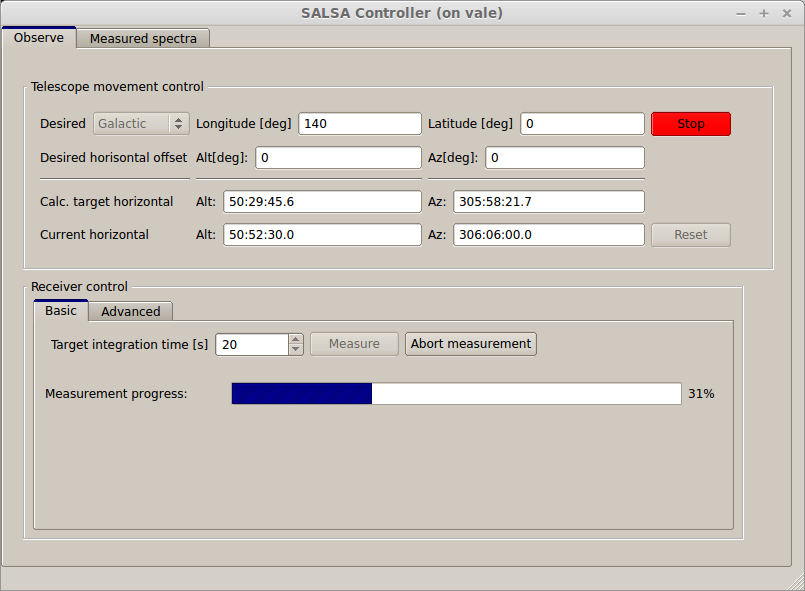
\includegraphics[width=\textwidth]{../figures/Controller_measure.png}
\end{center}
\caption{The telescope control program display when the telescope is measuring.}
\label{fig:controlmeasure}
\end{figure}

{\bf Note:} The telescope will, without any need for user interaction, divide
the specified integration time in two blocks. This is because in addition to
measure on the target (the signal you want), the telescope also needs to
measure itself (how the receiver disturbs the signal from space). The telescope
does this by shifting the measurement frequency away from hydrogen when it is measuring
itself. Finer control
of this \emph{switching} procedure can be found under the tab \emph{Advanced},
but don't change these values unless you know what you are doing. For normal users,
you only need to choose the total integration time in the \emph{Basic} tab.

\subsection{Measurement results}
\label{sect:inspect}
When a measurement is completed the resulting spectra is stored temporarily
within the control program.  To look at your measured spectra, click on the tab
\emph{Measured spectra} at the top of the program window. You will see a window
looking like Fig. ~\ref{fig:controlspectra}. On the left side is a list of all
spectra taken in this session (since you started the program). On the right
side is a graph over the currently marked spectrum. This plot is useful for a
quick inspection of the data. You can zoom using the buttons below the figure,
and if you hover with the mouse pointer in the figure the values for that
particular point in the graph will appear below the plot. 
\begin{figure}[ht]
\begin{center}
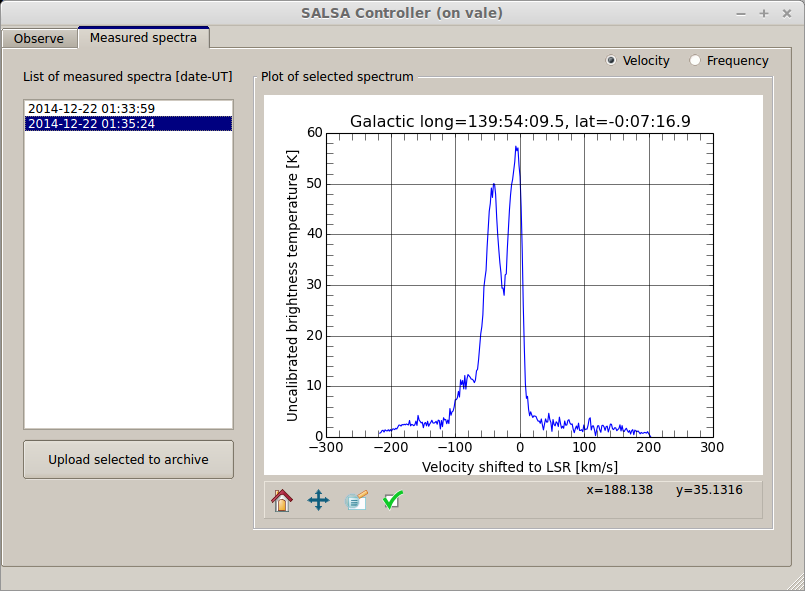
\includegraphics[width=0.9\textwidth]{../figures/Controller_spectra.png}
\end{center}
\caption{The tab \emph{Measured spectra} in the control program. To the left is
	a list of all measurements done in this session. The right plot shows the
	currently selected spectrum. You may select a different spectrum by clicking 
	the list. In the bottom left corner there is a button to save the
selected spectrum to the website data archive.}
\label{fig:controlspectra}
\end{figure}
While this is the easiest way to extract information from your measurement, it
may not be the most convenient. Instead, you may want to spend your time with
SALSA doing observations, and then do a careful analysis of your measurements
at another time. If so, you need to save your data.  In the bottom left corner
there is a button to save the selected spectrum to the online data archive.
After saving a measurement it will be available to you at any time via the
SALSA website, see Sect.  \ref{sect:archive}. The data should appear in the archive
within seconds of pressing the upload-button, so please check that you data has indeed been
uploaded before leaving the control program. Please note that if you do not
upload your measurement it will be deleted once you exit the control program.
\subsubsection{LSR correction}
The shift in frequency that one measures with SALSA is the result of 
a velocity difference between the telescope (the observer) and the target (source) 
along the line of sight. By default, the calculated radial velocity and measured frequency 
are corrected in SALSA for the observer's motion and expressed with respect to the Local-Standard-of-Rest (LSR) 
frame. This correction considers two main effects: the motion of the Sun relative 
to LSR and the orbital motion of the Earth relative to the Sun. LSR correction can be disabled on the \emph{Advanced} tab,
if one wishes not to use this option.
\subsubsection{RFI removal}
By default, median filtering is used in SALSA in order to filter away any radio frequency interference (RFI) 
present in the recorded signal. The idea of this filter is to go through the signal value by value and 
replace each value with the median of neighboring values. It is important to identify any RFI as it directly 
affects the obtained results (Fig.~\ref{fig:RFIremoval}). However, RFI removal can be disabled on
the \emph{Advanced} tab, if one wishes not to use this option.
\begin{figure}[ht]
\begin{center}
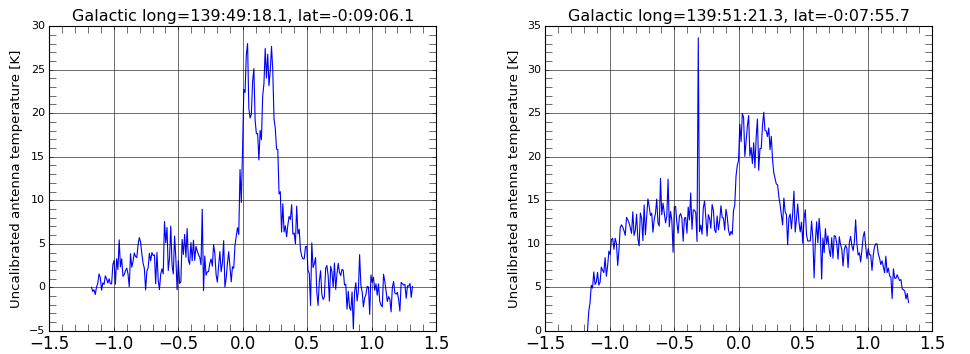
\includegraphics[width=\textwidth]{../figures/RFIremoval.png}
\end{center}
\caption{RFI removal in SALSA. The spectrum on the left side was obtained with default settings where RFI is filtered away. 
The other spectrum is a result of a subsequent measurement where the RFI removal option was disabled. One can identify there a narrow 
and strong peak that is a result of a disturbance generated by an external radio source. }
\label{fig:RFIremoval}
\end{figure}
\section{How to process archived data}
\label{sect:archiveprocess}
As mentioned in the previous section you may inspect your data directly within
the control program itself. This is the simplest option, but in some cases you
may want to do a more careful analysis offline, or you want to focus your 
observing time on getting data and do the processing later. In this section we 
briefly describe the most common ways to analyse the SALSA data you can download
from the archive at the SALSA webpage. 

\subsection{PNG: Images}
The PNG format is an image of the spectrum just as it looked in the control
program when you pressed the upload button. This is useful for a quick look,
but is less accurate than inspecting the data in the control program since you
cannot get the exact values from the graph in a simple way.  An accurate
analysis of your data will however probably require access to the actual
numbers, which is provided as TXT and FITS, see below.

\subsection{FITS: A common format for astronomical data}
A FITS file\footnote{Flexible Image Transport System (FITS) format.  A FITS
file contains two parts: a header followed by a binary record of the data.  The
binary table can be interpreted and displayed with FITS-reading software, for
example SalsaJ - see the SALSA website.} is a common format in astronomy.
This format provides the most functionality and meta-information. There are currently
two main ways to analyse FITS files from SALSA:

\begin{itemize}
\item \textbf{SalsaJ} was developed within the EU-HOU project.  SalsaJ can be
	used to analyse spectral data from the SALSA telscopes, but can also be
	used as a simple image editor and processor.  The main advantage of SalsaJ
	is its easy-to-use point-and-click interface. The main disadvantage is that
	reducing many spectra can be tedious. SalsaJ is available from the SALSA
	webpage {\url{http://vale.oso.chalmers.se/salsa/software}}, together with
	step-by-step instructions for opening FITS files from the webarchive.
\item \textbf{SalsaSpectrum} is a data reduction environment written
  in the popular mathematical software \textsc{\textsc{Matlab}} -
  aimed for reduction of data from SALSA Onsala, developed by Daniel
  Dahlin. The main advantage is that many spectra can be processed
  quickly. The main disadvantage is that it requires the user to have
  a working installation of Matlab, which is non-free software. Please note 
  that the observatory cannot provide Matlab licenses, but many university
  students have free access to Matlab. SalsaSpectrum is available from 
  the SALSA webpage {\url{http://vale.oso.chalmers.se/salsa/software}}, 
  together with step-by-step instructions for opening FITS files from the webarchive.
\end{itemize}

\subsection{TXT: Textfiles}
The TXT format contains the spectrum in plain text, i.e. as list of
velocity/intensity pairs. This is a simple format, and it is possible to use 
the file together with the PNG images to get accurate measurements of the peak
velocities. First get a rough estimate from the PNG-file, and then read the exact
values in the TXT file. If you know programming you may also write your own code to
show the TXT-files in your favourite language.

\subsection{Python}
If you are familiar with the programming language Python you can read the FITS
files using the library \emph{astropy.io.fits}. Please make sure to read the
VLSR-correction and reference pixels correctly. You can compare with the
results in the TXT and PNG-files. You may also skip the FITS files and read the
TXT-files directly with python. If you want to process many FITS files with Python,
you may find the scripts made by Michael Olberg, available at
https://github.com/molberg/salsa, to be a good starting point. 

\subsection{R}
If you are familiar with the programming language R you can read the FITS files
using R. You may find the scripts made by Michael Olberg, available at
https://github.com/molberg/salsa, to be a good starting point. 
